\documentclass{article}

\usepackage{algorithm,algpseudocode}
\usepackage[margin=1in]{geometry}
\usepackage{enumerate}
\usepackage{graphicx,subcaption}

\usepackage{amsfonts}
\def\R{{\mathbb R}}
\def\N{{\mathbb N}}

\title{Ford-Fulkerson Algorithm}
\author{CSCI 432}
\date{30 October 2019}

\begin{document}
\begin{figure}
\centering
\begin{subfigure}[b]{.45\textwidth}
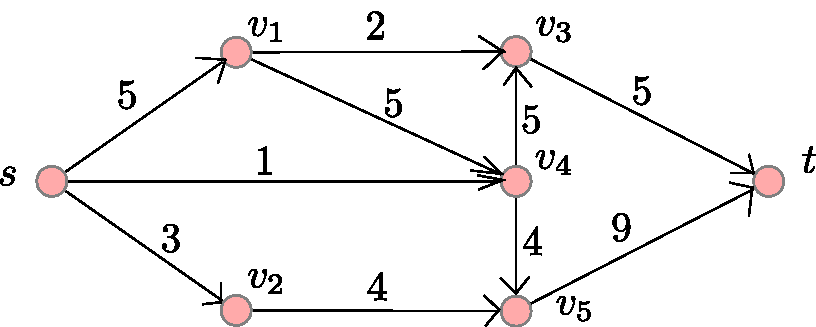
\includegraphics[width=\textwidth]{../figs/graph}\caption*{Flow}
\end{subfigure}
~~
\begin{subfigure}[b]{.45\textwidth}
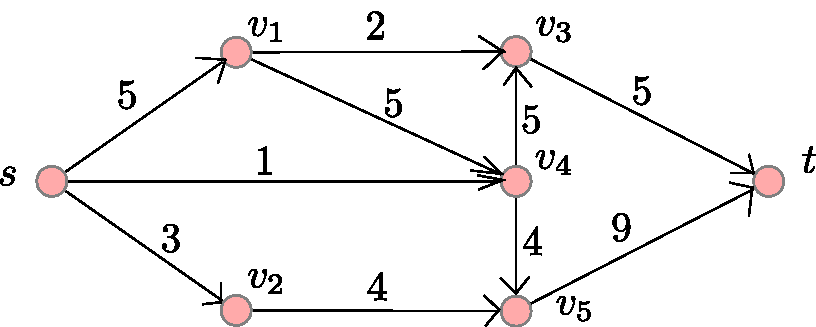
\includegraphics[width=\textwidth]{../figs/graph}\caption*{Residuals}
\end{subfigure}
\end{figure}

\begin{figure}
\centering
\begin{subfigure}[b]{.45\textwidth}
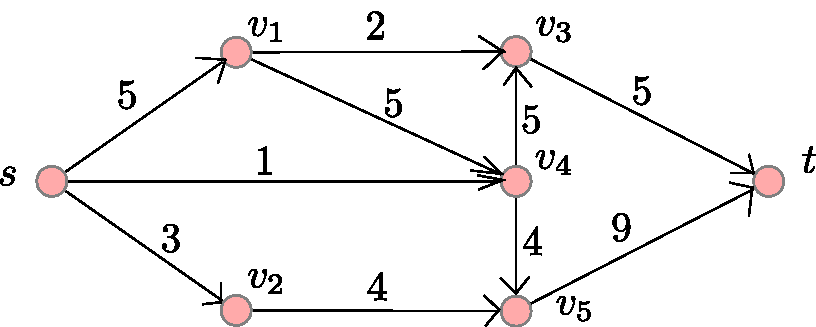
\includegraphics[width=\textwidth]{../figs/graph}\caption*{Flow}
\end{subfigure}
~~
\begin{subfigure}[b]{.45\textwidth}
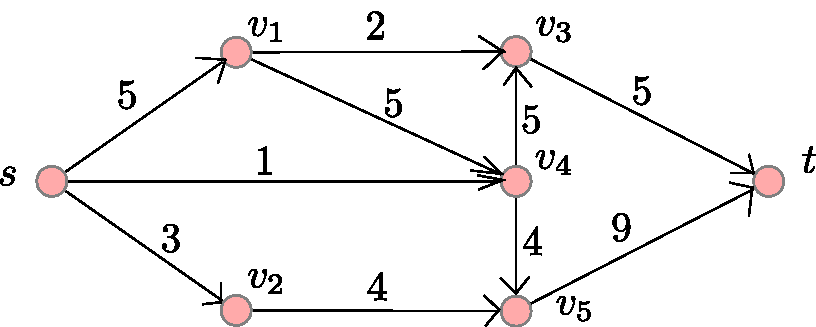
\includegraphics[width=\textwidth]{../figs/graph}\caption*{Residuals}
\end{subfigure}
\end{figure}

\begin{figure}
\centering
\begin{subfigure}[b]{.45\textwidth}
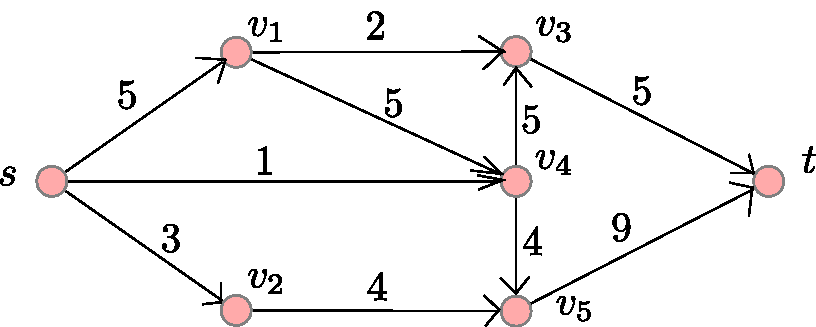
\includegraphics[width=\textwidth]{../figs/graph}\caption*{Flow}
\end{subfigure}
~~
\begin{subfigure}[b]{.45\textwidth}
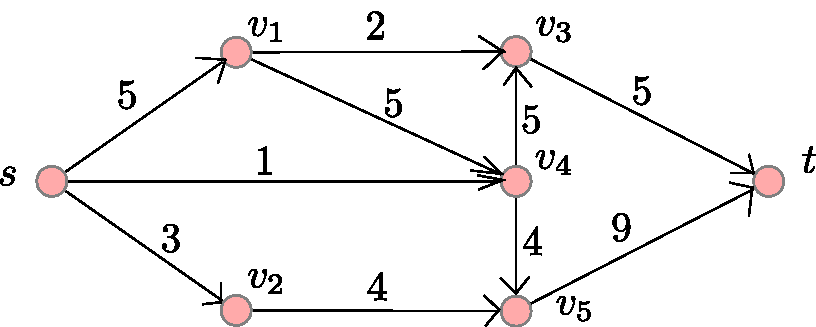
\includegraphics[width=\textwidth]{../figs/graph}\caption*{Residuals}
\end{subfigure}
\end{figure}


\begin{figure}
\centering
\begin{subfigure}[b]{.45\textwidth}
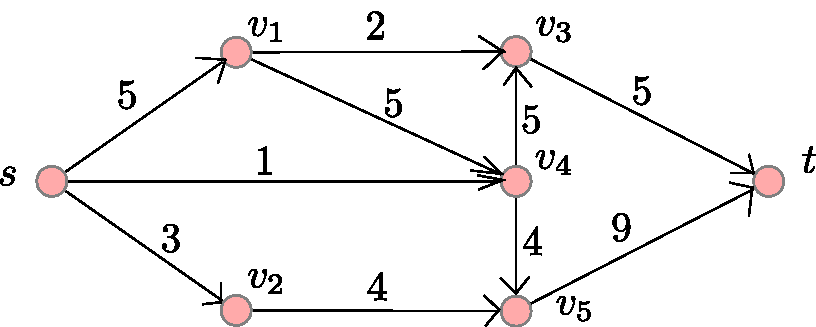
\includegraphics[width=\textwidth]{../figs/graph}\caption*{Flow}
\end{subfigure}
~~
\begin{subfigure}[b]{.45\textwidth}
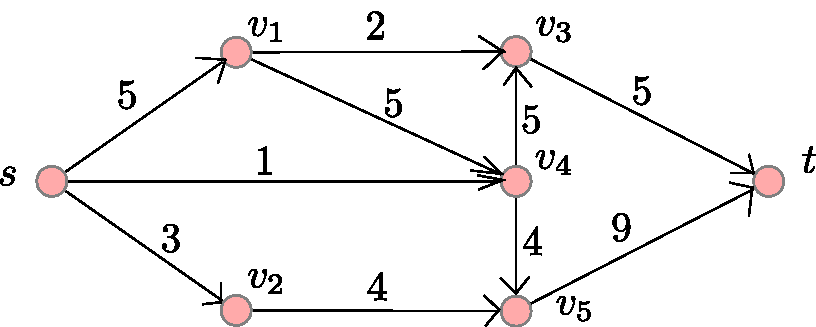
\includegraphics[width=\textwidth]{../figs/graph}\caption*{Residuals}
\end{subfigure}
\end{figure}


\begin{figure}
\centering
\begin{subfigure}[b]{.45\textwidth}
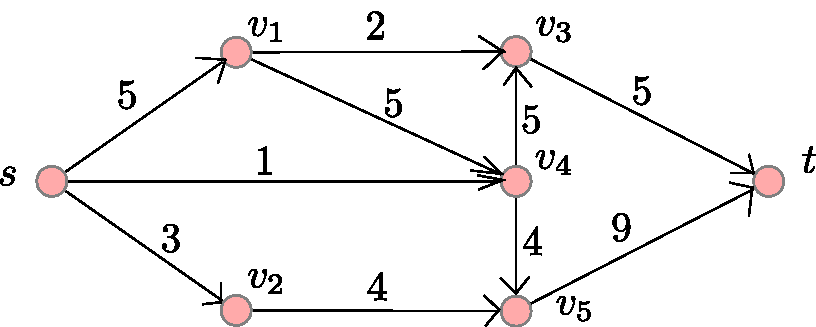
\includegraphics[width=\textwidth]{../figs/graph}\caption*{Flow}
\end{subfigure}
~~
\begin{subfigure}[b]{.45\textwidth}
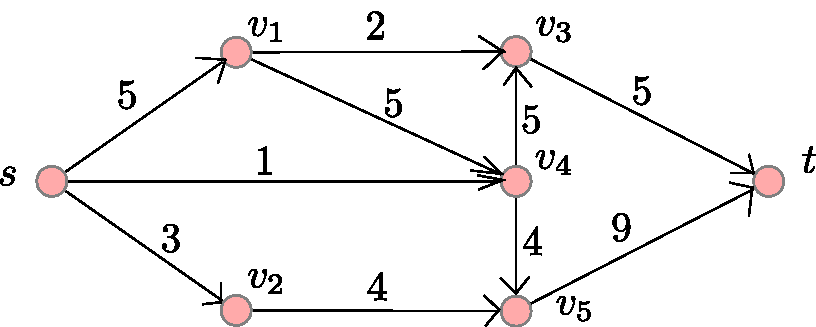
\includegraphics[width=\textwidth]{../figs/graph}\caption*{Residuals}
\end{subfigure}
\end{figure}


\begin{figure}
\centering
\begin{subfigure}[b]{.45\textwidth}
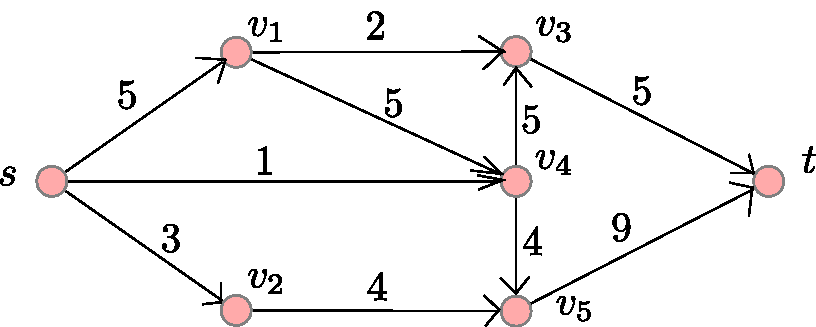
\includegraphics[width=\textwidth]{../figs/graph}\caption*{Flow}
\end{subfigure}
~~
\begin{subfigure}[b]{.45\textwidth}
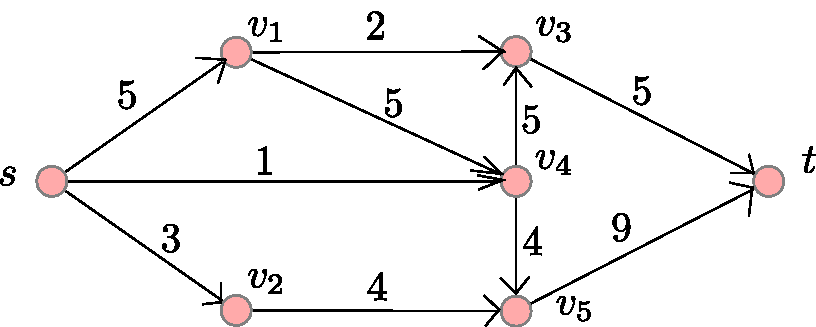
\includegraphics[width=\textwidth]{../figs/graph}\caption*{Residuals}
\end{subfigure}
\end{figure}



\begin{figure}
\centering
\begin{subfigure}[b]{.45\textwidth}
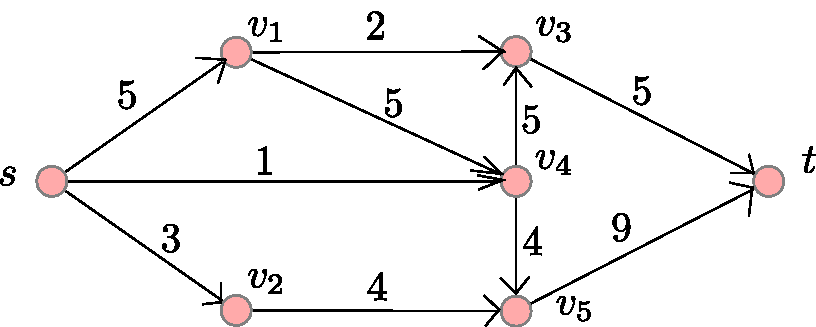
\includegraphics[width=\textwidth]{../figs/graph}\caption*{Flow}
\end{subfigure}
~~
\begin{subfigure}[b]{.45\textwidth}
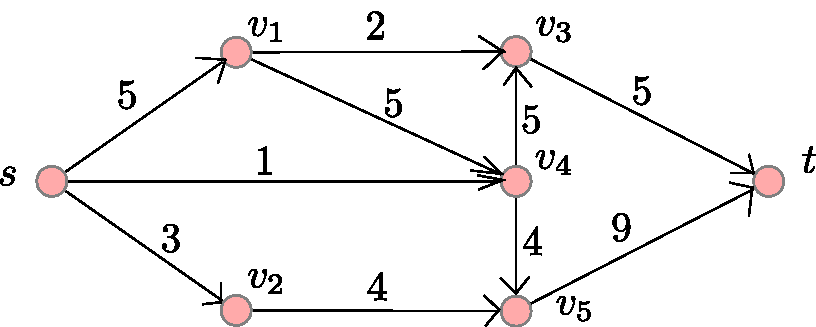
\includegraphics[width=\textwidth]{../figs/graph}\caption*{Residuals}
\end{subfigure}
\end{figure}


\begin{figure}
\centering
\begin{subfigure}[b]{.45\textwidth}
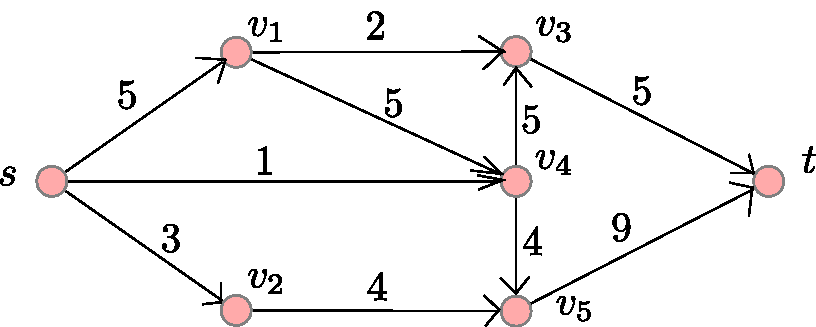
\includegraphics[width=\textwidth]{../figs/graph}\caption*{Flow}
\end{subfigure}
~~
\begin{subfigure}[b]{.45\textwidth}
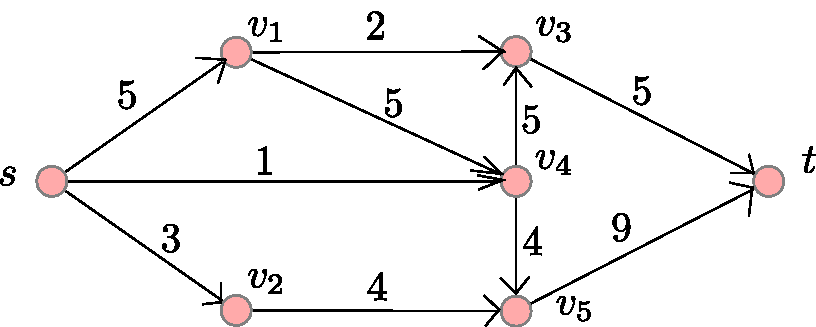
\includegraphics[width=\textwidth]{../figs/graph}\caption*{Residuals}
\end{subfigure}
\end{figure}

\begin{figure}
\centering
\begin{subfigure}[b]{.45\textwidth}
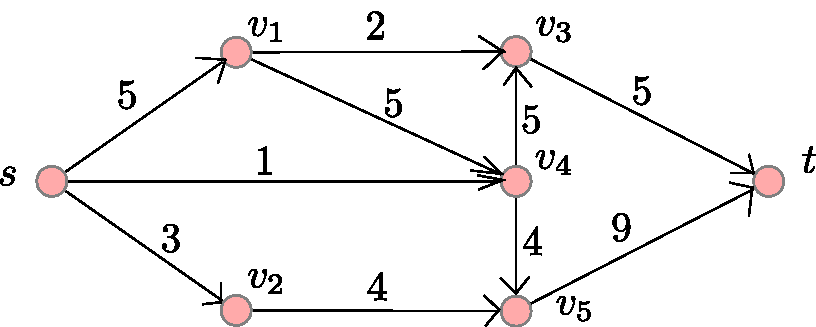
\includegraphics[width=\textwidth]{../figs/graph}\caption*{Flow}
\end{subfigure}
~~
\begin{subfigure}[b]{.45\textwidth}
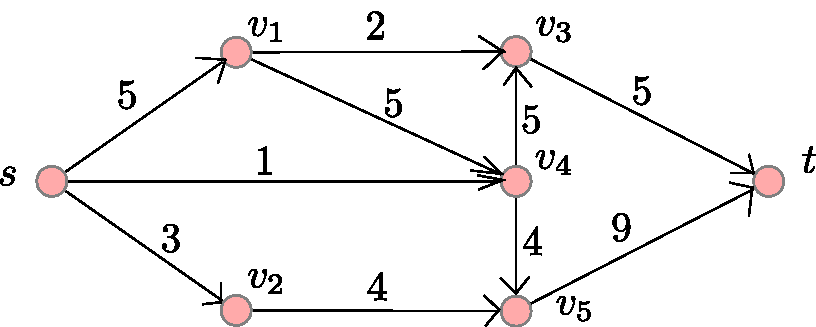
\includegraphics[width=\textwidth]{../figs/graph}\caption*{Residuals}
\end{subfigure}
\end{figure}



\begin{figure}
\centering
\begin{subfigure}[b]{.45\textwidth}
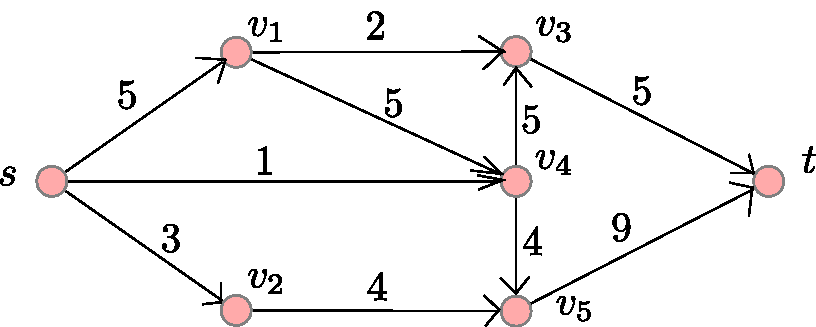
\includegraphics[width=\textwidth]{../figs/graph}\caption*{Flow}
\end{subfigure}
~~
\begin{subfigure}[b]{.45\textwidth}
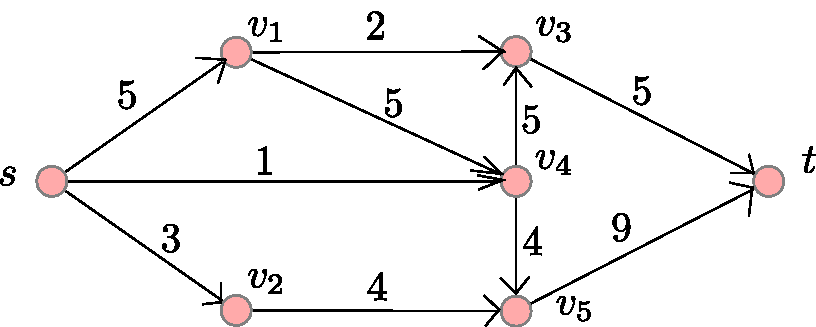
\includegraphics[width=\textwidth]{../figs/graph}\caption*{Residuals}
\end{subfigure}
\end{figure}



\end{document}